%!TEX TS-program = pdflatex
%!TEX root = ../main.tex
%!TEX encoding = UTF-8 Unicode


\section[YOHO model]{YOHO model}

	\begin{frame}{YOHO model}
			
		Presented in 2021, \textbf{YOHO}\footcite{Venkatesh_2022} is a novel and lightweight real-time algorithm for \textit{audio segmentation} and \textit{sound event detection}:
		\begin{itemize}
			\item it aims to detect acoustic classes and their temporal boundaries by treating the problem as a \textbf{regression task};
			\item inspired by \textit{YOLO} algorithm for machine vision.
		\end{itemize}
		
		\note{
			\dots			
		}		
		
	\end{frame}
	
	\begin{frame}{Input shape}
	
		The input of the network is a spectrogram
		\begin{figure}
			\centering
			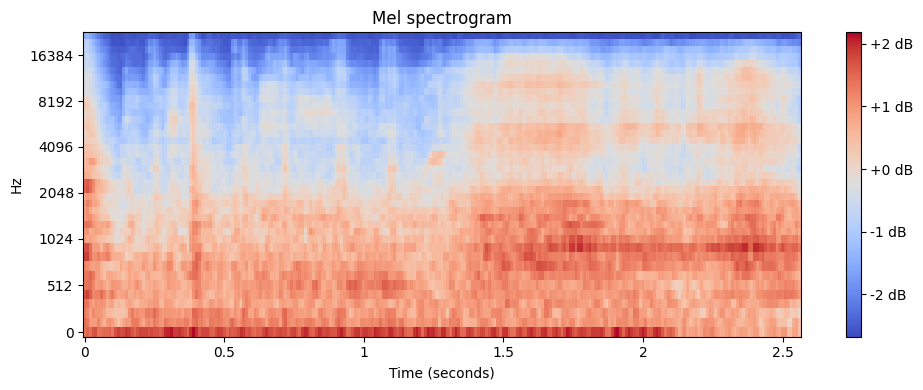
\includegraphics[width=.75\textwidth]{images/spectrogram.png}

			\caption{An example of mel-spectrogram.}
			\label{fig:spectogram}
		\end{figure}
	
		
		\note{
			\dots
		}
	\end{frame}
	
	
	\begin{frame}{Network Architecture}
		YOHO uses the MobileNet architecture as a backbone 
		
		\note{
			\dots
		}
	\end{frame}
	
	
	\begin{frame}{Output shape}
	
	\begin{figure}
			\centering
			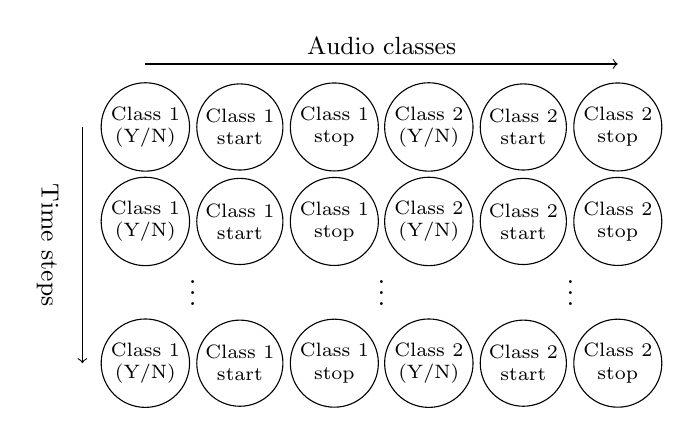
\begin{tikzpicture}[scale=.8]
			
				\draw [->,black] (1,6) -- node[midway,above]{\small Audio classes} (8.5,6);
				\draw [->,black] (0,5) -- node[midway,left,below=5pt,sloped]{\small Time steps} (0,1.25);
				
				\node[circle,draw,align=center,inner sep=0pt,text width=1cm,font = {\scriptsize}] at (1,5) {Class $1$\\(Y/N)};
				\node[circle,draw,align=center,inner sep=0pt,text width=1cm,font = {\scriptsize}] at (2.5,5) {Class $1$\\start};
				\node[circle,draw,align=center,inner sep=0pt,text width=1cm,font = {\scriptsize}] at (4,5) {Class $1$\\stop};

				\node[circle,draw,align=center,inner sep=0pt,text width=1cm,font = {\scriptsize}] at (5.5,5) {Class $2$\\(Y/N)};
				\node[circle,draw,align=center,inner sep=0pt,text width=1cm,font = {\scriptsize}] at (7,5) {Class $2$\\start};
				\node[circle,draw,align=center,inner sep=0pt,text width=1cm,font = {\scriptsize}] at (8.5,5) {Class $2$\\stop};


				\node[circle,draw,align=center,inner sep=0pt,text width=1cm,font = {\scriptsize}] at (1,3.5) {Class $1$\\(Y/N)};
				\node[circle,draw,align=center,inner sep=0pt,text width=1cm,font = {\scriptsize}] at (2.5,3.5) {Class $1$\\start};
				\node[circle,draw,align=center,inner sep=0pt,text width=1cm,font = {\scriptsize}] at (4,3.5) {Class $1$\\stop};

				\node[circle,draw,align=center,inner sep=0pt,text width=1cm,font = {\scriptsize}] at (5.5,3.5) {Class $2$\\(Y/N)};
				\node[circle,draw,align=center,inner sep=0pt,text width=1cm,font = {\scriptsize}] at (7,3.5) {Class $2$\\start};
				\node[circle,draw,align=center,inner sep=0pt,text width=1cm,font = {\scriptsize}] at (8.5,3.5) {Class $2$\\stop};

				\node[align=center] at (1.75,2.5) {$\vdots$};
				\node[align=center] at (4.75,2.5) {$\vdots$};
				\node[align=center] at (7.75,2.5) {$\vdots$};

				\node[circle,draw,align=center,inner sep=0pt,text width=1cm,font = {\scriptsize}] at (1,1.25) {Class $1$\\(Y/N)};
				\node[circle,draw,align=center,inner sep=0pt,text width=1cm,font = {\scriptsize}] at (2.5,1.25) {Class $1$\\start};
				\node[circle,draw,align=center,inner sep=0pt,text width=1cm,font = {\scriptsize}] at (4,1.25) {Class $1$\\stop};

				\node[circle,draw,align=center,inner sep=0pt,text width=1cm,font = {\scriptsize}] at (5.5,1.25) {Class $2$\\(Y/N)};
				\node[circle,draw,align=center,inner sep=0pt,text width=1cm,font = {\scriptsize}] at (7,1.25) {Class $2$\\start};
				\node[circle,draw,align=center,inner sep=0pt,text width=1cm,font = {\scriptsize}] at (8.5,1.25) {Class $2$\\stop};

			\end{tikzpicture}
			\caption{The YOHO output shape.}
			\label{fig:YOHOoutput}
		\end{figure}
		
	\end{frame}
	

	\begin{frame}{Loss Function}
		\begin{equation*}
			\mathcal{L}_{c}(\hat{y},y) = \begin{cases}
			(\hat{y}_1-y_1)^2+\\(\hat{y}_2-y_2)^2+(\hat{y}_3-y_3)^2 &\text{if $y_{1} = 1$}\\
			(\hat{y}_1-y_1)^2, &\text{if $y_1 = 0$}
			\end{cases}
		\end{equation*}
		
		where $y$ and $\hat{y}$ are the ground-truth and predictions respectively. $y_1 = 1$ if the acoustic class is present and $y_1 = 0$ if the class is absent. $y_2$ and $y_3$, which are the start and endpoints for each acoustic class are considered only if $y = 1$.
		In other words, $(\hat{y}_1-y_1)^2$ corresponds to \textbf{the classification loss} and $(\hat{y}_2-y_2)^2+(\hat{y}_3-y_3)^2$ corresponds to \textbf{the regression loss}.
		\note{
			\dots
		}
	\end{frame}
	
	\begin{frame}{Other Details}
		\dots
		
		\note{
			\dots
		}
	\end{frame}

\section[Work done and results]{Work done and results}	

	\begin{frame}[fragile]{Implementation challenges}
	
		Starting from the original paper, we implemented the system using PyTorch\footnote{All the code is available at \url{https://github.com/enstit/YOHO24}.},
		writing the code keeping in mind that it had to be \textbf{clear} and permit \textbf{reproducible tests}.
		
		\begin{lstlisting}[basicstyle=\tiny\ttfamily\color{white},language=bash,backgroundcolor=\color{black},caption={Training script parameters}, label={trainingParams},captionpos=b]
$ python3 -m yoho.train --help
usage: train.py [-h] [--name NAME] [--epochs EPOCHS] [--batch-size BATCH_SIZE] [--cosine-annealing]
[--autocast] [--spec-augment]

options:
  -h, --help            show this help message and exit
  --name NAME           The name of the model
  --epochs EPOCHS       The number of epochs to train the model
  --batch-size BATCH_SIZE
                        The batch size for training the model
  --cosine-annealing    Use cosine annealing learning rate scheduler
  --autocast            Use autocast to reduce memory usage
  --spec-augment        Augment the training data using SpecAugment
		\end{lstlisting}

		We used ORFEO\footnote{\url{https://www.areasciencepark.it/piattaforme-tecnologiche/data-center-orfeo/}} computational resources for the trainings of the models.
		
	\end{frame}
	
	\begin{frame}{Training results}
		\begin{figure}
			\centering
			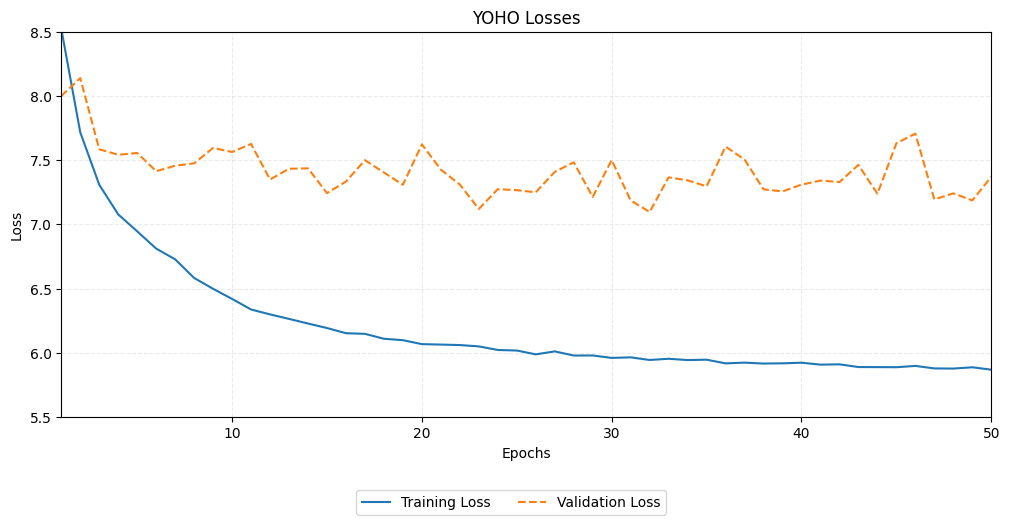
\includegraphics[width=.8\textwidth]{images/losses.png}

			\caption{Training and validation loss for YOHO model on UrbanSED dataset.}
			\label{fig:trainingLosses}
		\end{figure}
	\end{frame}
